%\chapter{About Figures}
%\label{chap-AboutFigures}
%\newthought{Figures in this chapter} are divided into two sections: 
%(1) figures from Tufte,
%(2) figures from other sources.
%
\section{Figures from Tufte}
\label{chap-Figures-Tufte}

\newthought{About the figures}  from Tufte:
\begin{itemize}
\item
a margin figure, {\tt fg-tufte-margin-helix}, Figure~\ref{fg-tufte-margin-helix}, 
\item
a normal-width figure, {\tt fg-tufte-normal-hilbertcurves}, Figure~\ref{fg-tufte-normal-hilbertcurves}, and
\item
a full-width figure, {\tt fg-tufte-wide-sine}, Figure~\ref{fg-tufte-wide-sine}.
\end{itemize}


\begin{marginfigure}[-50ex]%
  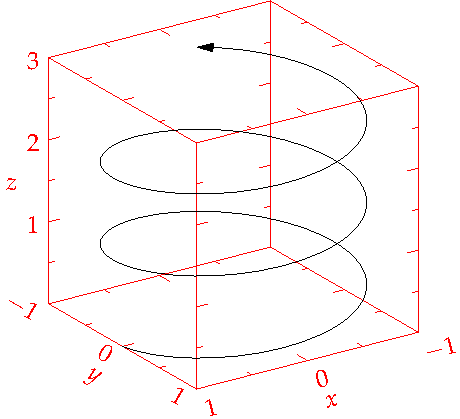
\includegraphics[width=\linewidth]{fg-tufte-margin-helix}
  \caption[Example file fg-tufte-margin-helix.tex]
  {This is a margin figure.  
    The helix is defined by 
    $x = \cos(2\pi z)$, $y = \sin(2\pi z)$, and $z = [0, 2.7]$. The figure was
    drawn using Asymptote (\url{http://asymptote.sf.net/}).}
  \label{fg-tufte-margin-helix}
\end{marginfigure}.






\begin{figure}[h!]%
  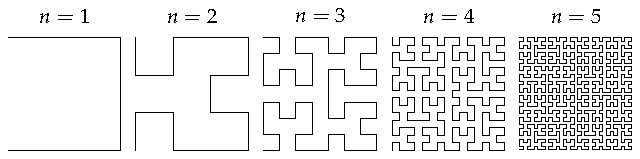
\includegraphics{fg-tufte-normal-hilbertcurves}
  \caption[Example file fg-tufte-normal-hilbertcurves.tex][6ex]
  {Hilbert curves of various degrees $n$. 
  \emph{Notice that this figure only takes up the main textblock width.}}
  \label{fg-tufte-normal-hilbertcurves}
\end{figure}

\lipsum[2]
\begin{figure*}[t!]
  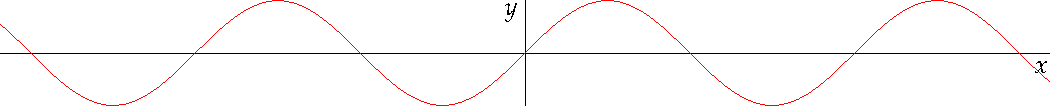
\includegraphics[width=\linewidth]{fg-tufte-wide-sine}%
  \caption[Example file fg-tufte-wide-sine.tex][2ex]
  {This graph shows $y = \sin x$ from about $x = [-10, 10]$.
  \emph{Notice that this figure takes up the full page width.}}%
  \label{fg-tufte-wide-sine}%
\end{figure*}